\chapter{Test Journal: Model Verification}\label{app:modelVerification}

\textbf{Date: 11/05/2017}

\subsection*{Purpose}
The purpose of this test journal is to get real measurements to verify the model, when moving the boat manually in the water.

%\subsection{Theory}
%By knowing the Force applied to the vessel and the acceleration, the added mass can be obtained by rearranging equation \autoref{eq:x_pos_model} and \autoref{eq:y_pos_model} to acquire the x and y components respectively.
%This assumes the force-input relationship of the actuators as well as the drag coefficients is known.

\subsection*{Equipment}
\begin{itemize}
	\item Vessel with all its components.
%	\item Emlid Reach RTK GPS
%	\item 2x INLINE 750 14.8V brushless DC-Motor
%	\item 2x Speed Controller +70 G3.5
%	\item ADIS16405BMLZ IMU
%	\item Ps3 Controller  
	\item External laptop.
\end{itemize}

%%%% Test Setup
\subsection*{Procedure}
\begin{enumerate}
	\item Turn on all equipment.
    \item Remotely log into the boat, when both, laptop and vessel's computer, are in the same network.
	\item Run the following nodes
		\begin{itemize}
			\item \lstinline[style=cinline]{/lli_node}
            \item \lstinline[style=cinline]{/sensor_node}
            \item \lstinline[style=cinline]{/gps_node}
			\item \lstinline[style=cinline]{/keyboard_teleop_node}
		\end{itemize}
    \item Record the following topics
        \begin{itemize}
            \item \lstinline[style=cinline]{/imu}
            \item \lstinline[style=cinline]{/gps_pos}
            \item \lstinline[style=cinline]{/lli_input}        
        \end{itemize}
	\item Move the vessel using the keyboard.
	\item Stop the recording.
    \item Bring the boat back to land and turn off the equipment.
    \item Process the data
\end{enumerate}

%\subsection{Error Sources}
%\begin{itemize}
%	\item Wind and Wave Disturbances
%	\item Measurement noise
%\end{itemize}

\subsection*{Results}
The results when applying two constant but different forces ($F1=-1$ N and $F1=12$ N), which produces a counterclockwise turn, can be seen below.
\begin{figure}[H]
    \captionbox 
    {   
        Position of the boat in the $x_\mathrm{n}$-$y_\mathrm{n}$ plane given by the GPS data.
        \label{fig:turn_app}
    }                                                                 
    {                                                                  
        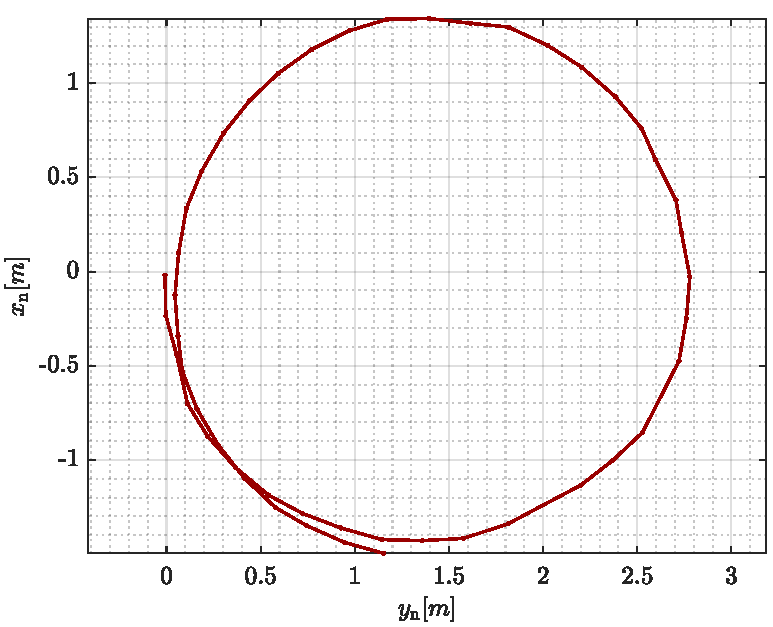
\includegraphics[width=.45\textwidth]{figures/turn_app}         
    }                                                                    
    \hspace{5pt}                                                          
    \captionbox  
    {      
        $x_\mathrm{n}$ and $y_\mathrm{n}$ with respect to time.
        \label{fig:turn_time_app}
    }                                                                          
    {
        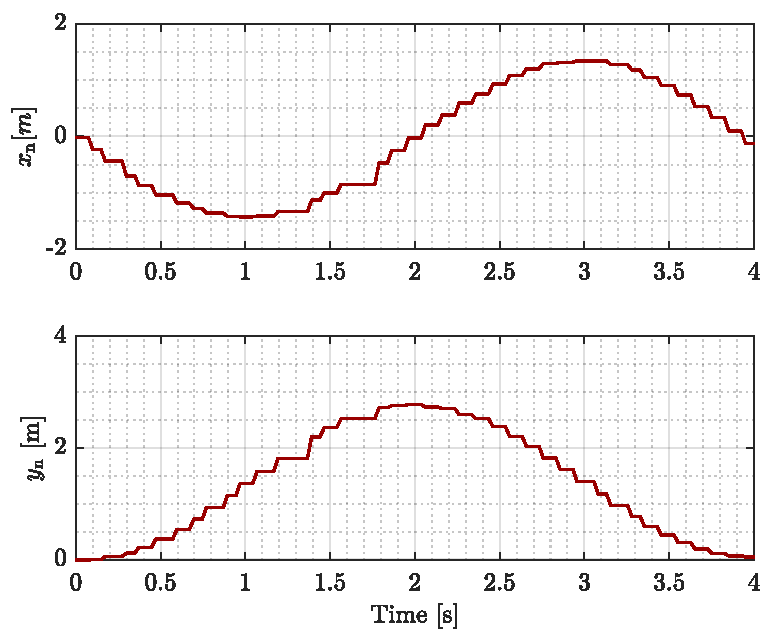
\includegraphics[width=.45\textwidth]{figures/turn_time_app}
    }
\end{figure}